\documentclass[12 pt]{article}
%%%%%%%%%%%%%%%%%%%%%%%%%%%%
%\topmargin 0.2in
%\textheight 10in
%\voffset -1.25in
%\textwidth 6.2in
%\parindent 0.25in
%\itemindent 0.in
%\leftmargin 0.5in
%\hoffset -0.8in

%\addtolength{\textwidth}{ain}
%\addtolength{\hoffset}{-bin}
%\addtolength{\textheight}{cin}
%\addtolength{\voffset}{cin}
%a=2b

\addtolength{\textwidth}{1.in}
\addtolength{\hoffset}{-.5in}
\addtolength{\textheight}{1.in}
\addtolength{\voffset}{-1.in}


%Packages
\usepackage{graphicx}
\usepackage[mathcal,mathscr]{eucal}
\usepackage{amsfonts}
\usepackage{mathrsfs}
\usepackage{amsmath, amsthm, amssymb,epsfig,amscd,multicol}
\usepackage{enumerate}
\usepackage{xcolor}
\usepackage{tikz}
\usetikzlibrary{arrows}
\usepackage{float}
\usepackage{caption}
\usepackage{subcaption}
\usepackage{tabu}
\usepackage{arydshln}
\usepackage{cancel}
%\usepackage{mathptmx}

%New Commands
\newcommand{\R}{\mathbb{R}}
\newcommand{\Z}{\mathbb{Z}}
\newcommand{\Q}{\mathbb{Q}}
\newcommand{\N}{\mathbb{N}}
\renewcommand{\P}{\mathscr{P}}
\newcommand{\set}[1]{\left\{#1\right\}}
\newcommand{\ds}{\displaystyle}
\newcommand{\diff}[2]{\frac{d #1}{d #2}}
\renewcommand{\subset}{\subseteq} 
\newcommand{\divides}{\! \mid \!}
\newcommand{\ndivides}{\! \nmid \!}
\newcommand{\mymod}[1]{ \ (\bmod \ #1)}
\newcommand{\esub}{\subseteq}
\newcommand{\rel}{\mathbin{R}}

\theoremstyle{definition}
\newtheorem{remark}{Remark}

\theoremstyle{plain}

\newtheoremstyle{mytheorem}% name of the style to be used
  {6pt}% measure of space to leave above the theorem. E.g.: 3pt
  {6pt}% measure of space to leave below the theorem. E.g.: 3pt
  {\itshape}% name of font to use in the body of the theorem
  {0pt}% measure of space to indent
  {\bfseries}% name of head font
  {.}% punctuation between head and body
  {5 pt plus 1pt minus 1pt}% space after theorem head; " " = normal interword space
  {}% Manually specify head
  
 	\theoremstyle{mytheorem}
  	\newtheorem{theorem}{Theorem}[section]%[numbering]
	\newtheorem{lemma}{Lemma}
	\newtheorem{cor}{Corollary}[section]
	\newtheorem{claim}{Claim}

\newtheoremstyle{myexample}% name of the style to be used
  {22pt}% measure of space to leave above the theorem. E.g.: 3pt
  {22pt}% measure of space to leave below the theorem. E.g.: 3pt
  {\normalfont}% name of font to use in the body of the theorem
  {0pt}% measure of space to indent
  {\bfseries}% name of head font
  {.}% punctuation between head and body
  {5 pt plus 1pt minus 1pt}% space after theorem head; " " = normal interword space
  {}% Manually specify head

	\theoremstyle{myexample}
	\newtheorem{example}{Example}[section]
	
\newtheoremstyle{mydefinition}% name of the style to be used
  {12pt}% measure of space to leave above the theorem. E.g.: 3pt
  {12pt}% measure of space to leave below the theorem. E.g.: 3pt
  {\normalfont}% name of font to use in the body of the theorem
  {0pt}% measure of space to indent
  {\bfseries}% name of head font
  {.}% punctuation between head and body
  {5 pt plus 1pt minus 1pt}% space after theorem head; " " = normal interword space
  {}% Manually specify head

	\theoremstyle{mydefinition}
	\newtheorem{definition}{Definition}
	\newtheorem*{definition*}{Definition}





\begin{document}
\pagenumbering{gobble}
\begin{center}
\textbf{P.~19 Injections and Surjections and Bijections...Oh My!}
\end{center}

While functions can have any number of various properties, none are more important than injectivity, surjectivity, and bijectivity.  More commonly you know of injective as ``one-to-one'' and surjective as ``onto.''

\begin{center}
\fbox{\parbox{5.5in}{Goals:
\begin{itemize}
\item Define injection, surjection, and bijection
\item Prove that functions have these properties
\end{itemize}
}}
\end{center}

You've undoubtedly heard the terms ``one-to-one'' and ``onto'' at some point in your mathematics education, but to be fair you probably don't have a strong grasp on these concepts.  Part of this is because the functions that you normally see that are defined on the real numbers make these concepts more complicated than they need to be.  Let's start with injectivity.


\section{Injections}
\begin{definition*}  Let $f: A \to B$.  For $a_1,a_2 \in A$, if $f(a_1)=f(a_2)$ implies that $a_1=a_2$, then we say that $f$ is \textit{injective} or \textit{one-to-one}.
\end{definition*}

What this definition says is that a function is injective if any output that gets hit only gets hit by one input.  So
\begin{multicols}{4}
This happens:

\resizebox{1.2in}{!}{
\begin{tikzpicture}
\draw (0,0) rectangle (2,4);
\node at (1,1){$\bullet$};
\node at (1,3){$\bullet$};
\draw (4,0) rectangle (6,4);
\node at (5,1){$\bullet$};
\node at (5,3){$\bullet$};
\draw[->] (1.2,1)--(4.8,1);
\draw[->] (1.2,3)--(4.8,3);
\node at (1,-.25){$A$};
\node at (5,-.25){$B$};
\node at (3,3.5){$f$};
\end{tikzpicture}}

Or this happens:

\resizebox{1.2in}{!}{
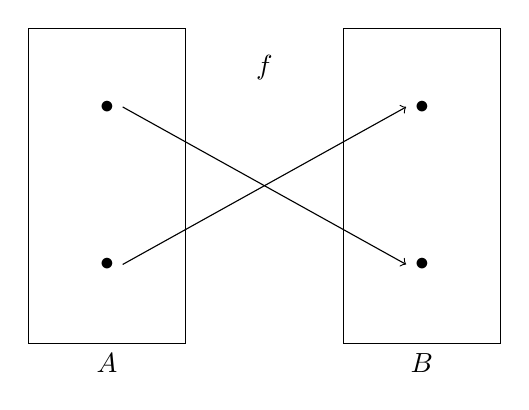
\begin{tikzpicture}
\draw (0,0) rectangle (2,4);
\node at (1,1){$\bullet$};
\node at (1,3){$\bullet$};
\draw (4,0) rectangle (6,4);
\node at (5,1){$\bullet$};
\node at (5,3){$\bullet$};
\draw[->] (1.2,1)--(4.8,3);
\draw[->] (1.2,3)--(4.8,1);
\node at (1,-.25){$A$};
\node at (5,-.25){$B$};
\node at (3,3.5){$f$};
\end{tikzpicture}}

Not this:

\resizebox{1.2in}{!}{
\begin{tikzpicture}
\draw (0,0) rectangle (2,4);
\node at (1,1){$\bullet$};
\node at (1,3){$\bullet$};
\draw (4,0) rectangle (6,4);
\node at (5,1){$\bullet$};
\node at (5,3){$\bullet$};
\draw[->] (1.2,1)--(4.8,1);
\draw[->] (1.2,3)--(4.8,1.2);
\node at (1,-.25){$A$};
\node at (5,-.25){$B$};
\node at (3,3.5){$f$};
\end{tikzpicture}}

Nor this:

\resizebox{1.2in}{!}{
\begin{tikzpicture}
\draw (0,0) rectangle (2,4);
\node at (1,1){$\bullet$};
\node at (1,3){$\bullet$};
\draw (4,0) rectangle (6,4);
\node at (5,1){$\bullet$};
\node at (5,3){$\bullet$};
\draw[->] (1.2,1)--(4.8,2.8);
\draw[->] (1.2,3)--(4.8,3);
\node at (1,-.25){$A$};
\node at (5,-.25){$B$};
\node at (3,3.5){$f$};
\end{tikzpicture}}
\end{multicols}

A function might be one-to-one as opposed to two-to-one.  The common function $f(x)=x^2$ is two-to-one because each output of the function gets hit by two inputs.  For instance $4$ gets hit by $2$ and $-2$, $9$ gets hit by $3$ and $-3$, etc.  By definition, if something is one-to-(a number bigger than one) then it's not a function.  We call such things \textit{maps}.

\begin{enumerate}
\item Is the Birthmonth function injective for your group?  Why or why not?

\vspace{2in}

\item Is the archery function injective?  Explain your answer.

\vspace{2in}
\end{enumerate}

The definition given above for injection is the most common because it's the simplest to understand (that's debatable).  The next definition requires that you recall what the range of $f$, denoted $R_f$, is.

\begin{enumerate} \setcounter{enumi}{2}
\item For $f: A \to B$, what is $R_f$?  Give the name of $R_f$ and its description in set-builder notation.

\vspace{2in}

\end{enumerate}

\begin{definition*}  The function $f: A \to B$ is \textit{injective} if for all $b \in R_f$ there exists a unique $a \in A$ such that $f(a)=b$.
\end{definition*}

The benefit of this new definition is that it tells us that to prove a function is injective, we need to write a uniqueness proof.

\begin{enumerate} \setcounter{enumi}{3}
\item How do you prove something is unique?

\vspace{1.5in}

\item Read the following injection claim and proof and justify the steps.
\begin{claim}
The function $f: \R \to \R$ given by $f(x)=-2x+1$ is injective.
\end{claim}
\begin{proof}  Let $f: \R \to \R$ be given by $f(x) = -2x+1$ and for sake of contradictions suppose there exists distinct real numbers $a$ and $b$ such that $f(a)=f(b)$.  Then
	\begin{align*}
	-2a+1 &= -2b+1 \\
	-2a &= -2b \\
	a &= b.
	\end{align*}
	This is a contradiction, so $f(a) \neq f(b)$ when $a \neq b$.  Therefore $f$ is injective.
\end{proof}
\item Prove that $g: \R \to \R$ given by $g(x) = x^3$ is injective.

\vspace{2.5in}
\item Prove that $h: \R^+ \to \R$ given by $h(t) = \sqrt{t}$ is injective.

\vspace{2.5in}
\item Prove that $s: \R \to \R$ given by $s(t) = \sin(t)$ is not injective.

\vspace{2.5in}
\end{enumerate}

\section{Surjections}

The idea of a surjection (or onto function) is actually really simple.  Dr.~Wright is convinced that the only reason anyone ever struggles with it is because they weren't taught the difference between a range and a codomain.  Two equivalent definitions for surjective follow.  The first one tells us what surjective really means, but the second tells us how to prove a function is surjective.
\begin{definition*}  Let $f: A \to B$.  Then $f$ is \textit{surjective} or \textit{onto} if $R_f = B$.
\end{definition*}

\begin{definition*}  Let $f: A \to B$.  Then $f$ is \textit{surjective} or \textit{onto} if for all $b \in B$, there exists $a\in A$ such that $f(a)=b$.
\end{definition*}

In pictures,
\begin{multicols}{2}
If we have this\\

\resizebox{2in}{!}{
\begin{tikzpicture}
\draw (0,0) rectangle (2,4);
% \node at (1,1){$\bullet$};
% \node at (1,3){$\bullet$};
\draw (4,0) rectangle (6,4);
%\node at (5,1){$\bullet$};
\node at (5,3){$\bullet$};
\node at (5,2.7){$b$};
%\draw[->] (1.2,1)--(4.8,1);
%\draw[->] (1.2,3)--(4.8,1.2);
\node at (1,-.25){$A$};
\node at (5,-.25){$B$};
%\node at (3,3.5){$f$};
\end{tikzpicture}}

Then we have this\\

\resizebox{2in}{!}{
\begin{tikzpicture}
\draw (0,0) rectangle (2,4);
\node at (1,1){$\bullet$};
\node at (1,.7){$a$};
%\node at (1,3){$\bullet$};
\draw (4,0) rectangle (6,4);
%\node at (5,1){$\bullet$};
\node at (5,3){$\bullet$};
\node at (5,2.7){$b$};
\draw[->] (1.2,1)--(4.8,2.8);
%\draw[->] (1.2,3)--(4.8,1.2);
\node at (1,-.25){$A$};
\node at (5,-.25){$B$};
\node at (3,3.5){$f$};
\end{tikzpicture}}
\end{multicols}

From these definition, we can tell that proving that a function is surjective means writing an existence proof.

\begin{enumerate}
\item Read the following proof that $f(x)=\sqrt[3]{x}$ is surjective and answer the questions that follow.
	\begin{proof}
	Suppose $f(x) = \sqrt[3]{x}$ and suppose $b \in \R$.  Let $a=b^3$.  Then $f(a)=f(b^3)=\sqrt[3]{b^3}=b$.  Thus, for all $b \in \R$, there exists $a \in \R$ such that $f(a)=b$.
	\end{proof}
	\begin{enumerate}
	\item Does the proof tell us where letting $a=b^3$ came from?  Should the proof tell us how to find the appropriate $a$?
	
	\vspace{1.5in}
	
	\item Remember that one way to think about a surjection is $R_f=B$.  The proof has shown that $B \esub R_f$.  Why doesn't it need to show that $R_f \esub B$?
	
	\vspace{2in}
	\end{enumerate}

\item Prove that $f: \R \to \R$ given by $f(x) = 5x+7$ is surjective.

\vspace{2.5in}  

\item Prove that $g: \Z-\set{0} \to \N$ given by $g(x)=x^2$ is surjective.

\vspace{2.5in}

\item Another way to say that function is surjective is to say is ``maps $A$ onto $B$.''  For a function $f$ with domain $D$, is it true that $f$ maps $D$ onto $R_f$?  Why or why not?

\vspace{2in}
\end{enumerate}

\section{Bijectivity}

The best thing about bijections is that they're really nothing new.

\begin{definition*}  For $f: A \to B$, $f$ is a \textit{bijection} if it is both injective and surjective.
\end{definition*}

\begin{enumerate}
\item For each of the following, determine if the function is an injection, surjection, or bijection.  Prove your conclusion either with an appropriate proof or counterexample.
	\begin{enumerate}
	\item When $f: \R \to \R$ is given by $f(x)=e^x$.
	
	\vspace{3.5in}
	
	\item When $f: D \subset \R \to \R$ is given by $f(x)=\tan(x)$.
	
	\vspace{4in}
	
	\item When $f: \Z \to \set{0,1,\ldots,9}$ is given by $f(x) = 2x \mymod{10}$.
	
	\vspace{3.5in}
	
	\item When $f: \Z \to \set{0,1,2}$ is given by $f(x) = 2x \mymod{3}$.
	\end{enumerate}
\end{enumerate}
\end{document}




